\chapter{Tamandua}
\section{Présentation}
Pour achever notre travail sur les algorithmes précédement exposés, nous avons
dû concevoir une architecture permettant de les implémenter, de leur fournir des
données à traiter et enfin de visualiser le résultat et les comparer entre eux.
\section{Architecture}
Dans un soucis d'efficacité de programmation et de réutilisabilité, l'ensemble
des problèmes à été implementé au sein d'une même architecture générique, celle-ci
se divise en plusieurs couches superposées:
\begin{itemize}
   \item td\_base contient des éléments fondamentaux n'ayant aucune spécifité
   vis-à-vis du projet, tel que la gestion mémoire et des algorithmes génériques.
   \item td\_core est le noyau de calcul, c'est dans cette partie que se trouve
   tout le code spécifique de génération de données, de répartition des calculs
   et d'extraction de résultats.
   \item les problèmes sont des bibliothèques dynamiques chargées à l'exécutions
   par le td\_core ils exportent une interface commune permettant d'informer le
   noyau des types de tâches qui l'intéresse, du nom du problème et des
   différents algorithmes de résolutions existants pour résoudre un problème,
   ces différents algorithmes sont appelés stratégies.
   \item l'interface graphique, au sommet de tout, charge la bibliothèque du 
   noyau et communique avec pour permettre à l'utilisateur de configurer la
   génération de donnée, et recevoir le résultat des calculs pour en faire
   quelque chose de lisible.
\end{itemize}
\section{Détails d'implémentation}
Le tout est réalisé en C sauf l'interface graphique en Qt programmée en C++.
Le noyau implémente un mécanisme simple de parallélisme basé sur les Posix Threads.
Ce mécanisme est à double usage, il permet d'une part de communiquer de manière
asynchrone avec les interfaces graphiques afin de ne pas provoquer de bloquage
inesthétique de l'interface pendant les calculs. D'autre part en associant une
liste d'attente de tâches et un ensemble de Threads, il profite des architectures
multi-thread et multi-coeur que l'on trouve de plus en plus même dans le grand
public.
\section{Génération de tâches}
La conception de la génération d'ensemble de tâches à faire traiter par un
algorithme n'a pas été triviale, plusieux choix s'offraient à nous avec différents
compromis de flexibilité et d'ergonomie, nous avions par exemple :
\begin{itemize}
   \item Une liste de tâche entièrement éditable à la main, précise mais extrèmement
   fastidieuse pour de grands ensembles ou pour en produire de nombreuses différentes.
   \item Un générateur aléatoire simple et homogène.
   \item La possibilité pour l'utilisateur de spécifier des contraintes sous forme
   d'équations, peut-être idéal pour tester directement certaines configurations
   connues mais d'implémentation difficile et peu intuitive lorsqu'on doit créer
   ces contraintes.
\end{itemize}
Nous avons finalement opté pour un mélange des deux premières solutions, en
employant une liste éditable de générateurs aléatoires, chacun pouvant être
configuré différemment, chaque générateur produit une population de tâches,
le tout est réunit pour faire un grand ensemble qui est alors envoyé aux
stratégies de résolution. On peut pousser l'extrème en employant autant de
populations que de tâches et en limitant chacune à une seule tâche pour reproduire
la première solution et à l'inverse n'avoir qu'une population et reproduire la seconde
solution.
\section{Présentation des interfaces graphiques}
\subsection{Gamandua}
Gamandua est l'interface en C utilisant la bibliothèque graphique GTK, elle est
constituée d'une fenêtre unique. En haut une barre d'outils permet de choisir 
le problème, la stratégie de résolution et le nombre de machines le cas échéant.
On y trouve aussi les contrôles principaux permettant d'exécuter des calculs,
d'exporter une image du résultat ainsi que l'aide. Sur le côté se trouve la
configuration des générateurs aléatoires de tâches, avec le choix du nombre
de populations et des paramètres séparés sur chacune.
\begin{center}
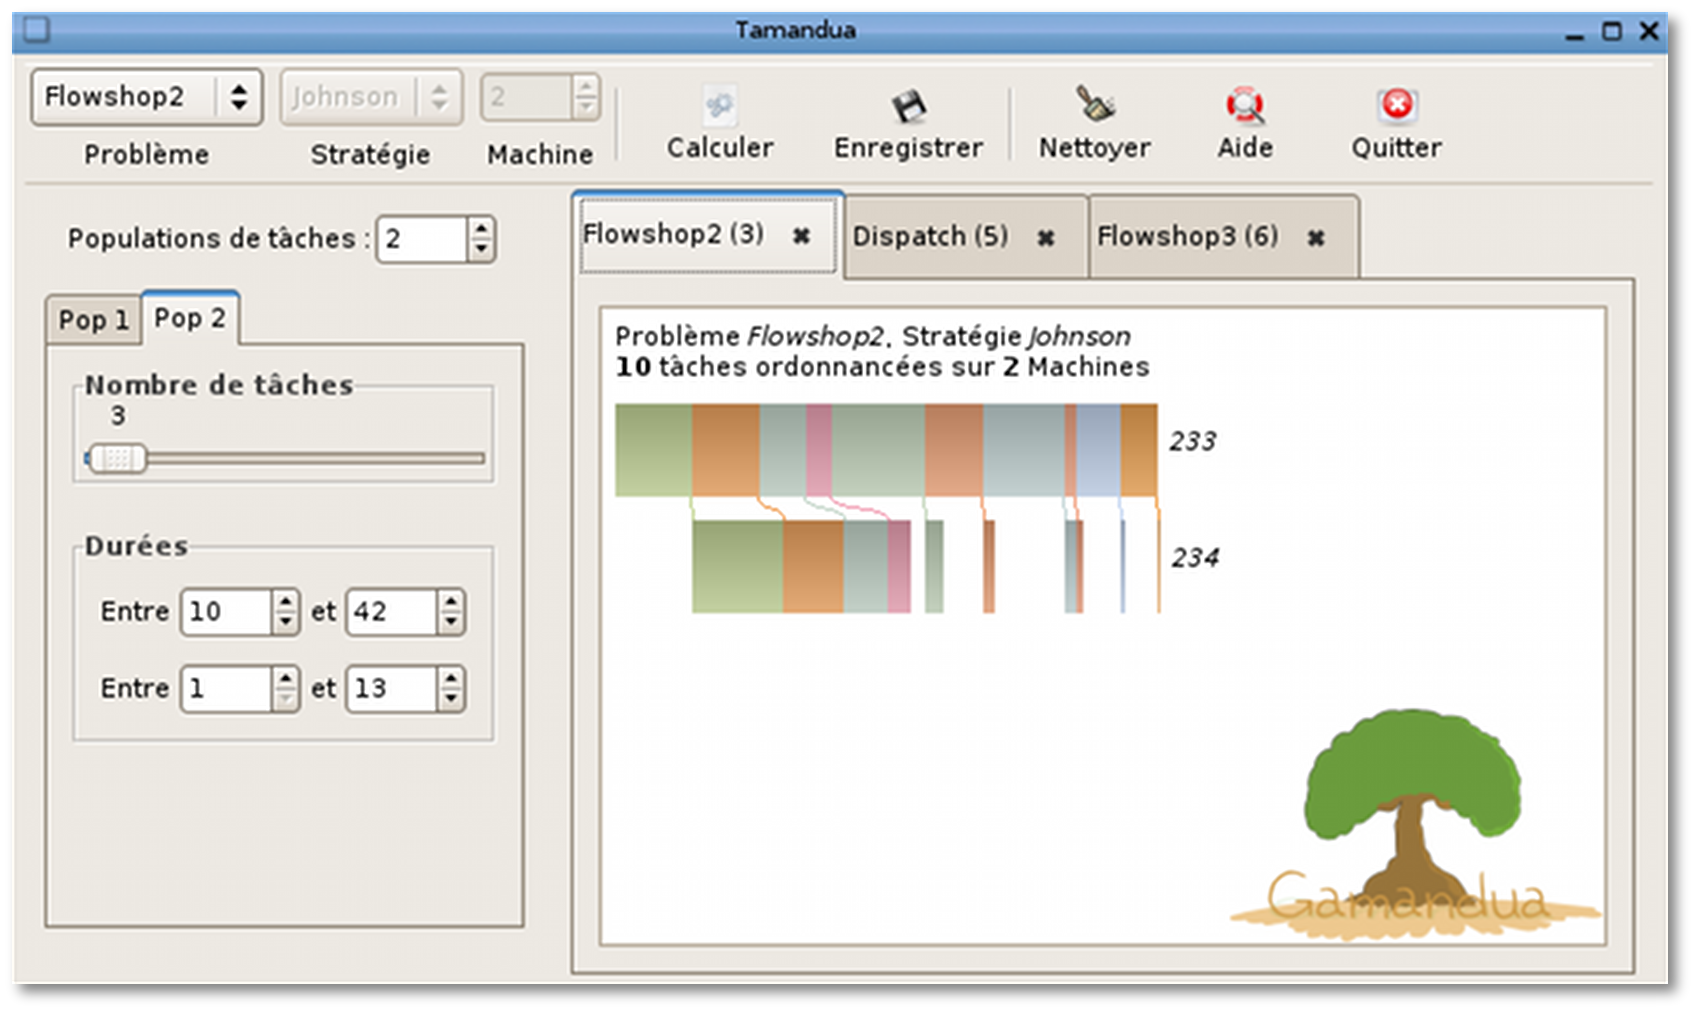
\includegraphics{gamandua.png}
\end{center}
Enfin le plus important au
milieu, les résultats des calculs, présentés sous forme de barres horizontales.
Dans le sens principal se trouve le temps, et à la verticale les différentes
machines, chaque tâche est représentée par un rectangle de couleur. La couleur
n'a aucune signification logique si ce n'est tenter de rendre le graphique
lisible. en cliquant sur les tâches une petite bulle s'affiche comportant des
informations supplémentaires. Plusieurs graphiques peuvent être conservés
simultanément grâce à un dispositif d'onglets en haut de l'affichage. Grâce au
bouton idoïne dans la barre d'outil, on peut exporter cette image en png si
on souhaite par exemple l'intégrer à un rapport ou la conserver en lieu sûr.
